% !TeX encoding = UTF-8
% !TeX program = xelatex
% !TeX spellcheck = en_US\part{title}

\documentclass{cjc}

\usepackage{booktabs}
\usepackage{algorithm}
\usepackage{algorithmic}
\usepackage{siunitx}

\classsetup{
  % 配置里面不要出现空行
  title        = {动量梯度法优化的置信规则库推理方法},
  title*       = {Belief rule base inference method based on gradient descent with  momentum},
  authors      = {
    author1 = {
      name         = {作者名},
      name*        = {NAME Name-Name},
      affiliations = {aff1},
      biography    = {性别,xxxx年生,学位(或目前学历),职称,是/否计算机学会(CCF)会员(提供会员号),主要研究领域为*****、****.},
      % 英文作者介绍内容包括:出生年, 学位(或目前学历), 职称, 主要研究领域(与中文作者介绍中的研究方向一致).
      biography*   = {Ph.D., asociate profesor. His/her research interests include ***, ***, and ***.},
      email        = {**************},
      phone-number = {……},  % 第1作者手机号码(投稿时必须提供,以便紧急联系,发表时会删除)
    },
    author2 = {
      name         = {作者名},
      name*        = {NAME Name},
      affiliations = {aff2, aff3},
      biography    = {性别,xxxx年生,学位(或目前学历),职称,是/否计算机学会(CCF)会员(提供会员号),主要研究领域为*****、****.},
      biography*   = {英文作者介绍内容包括:出生年, 学位(或目前学历), 职称, 主要研究领域(与中文作者介绍中的研究方向一致).},
      email        = {**************},
    },
    author3 = {
      name         = {作者},
      name*        = {NAME Name-Name},
      affiliations = {aff3},
      biography    = {性别,xxxx年生,学位(或目前学历),职称,是/否计算机学会(CCF)会员(提供会员号),主要研究领域为*****、****.},
      biography*   = {英文作者介绍内容包括:出生年, 学位(或目前学历), 职称, 主要研究领域(与中文作者介绍中的研究方向一致).},
      email        = {**************},
      % 通讯作者
      corresponding = true,
    },
  },
  % 论文定稿后,作者署名、单位无特殊情况不能变更。若变更,须提交签章申请,
  % 国家名为中国可以不写,省会城市不写省的名称,其他国家必须写国家名。
  affiliations = {
    aff1 = {
      name  = {单位全名\ 部门(系)全名, 市(或直辖市) 国家名\ 邮政编码},
      name* = {Department of ****, University, City ZipCode, Country},
    },
    aff2 = {
      name  = {单位全名\ 部门(系)全名, 市(或直辖市) 国家名\ 邮政编码},
      name* = {Department of ****, University, City ZipCode},
    },
    aff3 = {
      name  = {单位全名\ 部门(系)全名, 市(或直辖市) 国家名\ 邮政编码},
      name* = {Department of ****, University, City ZipCode, Country},
    },
  },
  abstract     = {
    扩展置信规则库在传统置信规则库基础上引入规则前件属性置信分布结构,使用训练数据构建规则库的规则,该方法简单高效。但在训练数据数目较多时需要进行规则约简或使用数据结构优化规则的存储与激活过程。为了解决这些问题,本文对传统扩展置信规则库的结构进行简化,取消规则前件属性置信分布形式,引入高斯函数优化规则激活权重计算过程,最终使用动量优化的随机梯度下降法训练置信规则库推理系统的参数。在实验分析中,通过拟合多极值非线性函数验证该方法的有效性,并在多个公共数据集比较该方法与其他置信规则库参数训练方法,实验结果表明该方法在简化置信规则库结构、优化激活过程的同时提升了推理的精度。
  },
  abstract*    = {
  	Extended belief rule base introduce the belief structure of rule antecedent attributes based on the traditional belief rule base, and use the training data to construct the rules of the rule base. This method is simple and efficient. However, when the number of training data is large, it is necessary to perform rule reduction or use data structure to optimize the storage and activation process of rules. In order to solve these problems, this paper simplifies the structure of the traditional extended belief rule base, cancels the pre-attribute attribute belief distribution form, introduces the Gaussian function to optimize rule activation weight calculation method, and finally uses the momentum-optimized stochastic gradient descent method to train the belief rule base parameters. In the experimental analysis, the method is validated by fitting a multi-extremal nonlinear function, and the method is compared with other belief rule base parameter training methods in multiple public data sets. Experimental results show that the method simplifies the structure of the belief rule base and optimizes the activation process while improving the accuracy of inference.
  },
  % 中文关键字与英文关键字对应且一致,应有5-7个关键词,不要用英文缩写
  keywords     = {置信规则库, 结构优化, 参数训练, 梯度法, 动量优化},
  keywords*    = {belief rule base, structure optimization, Parameter training, Gradient method, Momentum optimization},
  grants       = {
    本课题得到……基金中文完整名称(No.项目号)、
    ……基金中文完整名称(No.项目号)、
    ……基金中文完整名称(No.项目号)资助.
  },
  % clc           = {TP393},
  % doi           = {10.11897/SP.J.1016.2020.00001},  % 投稿时不提供DOI号
  % received-date = {2019-08-10},  % 收稿日期
  % revised-date  = {2019-10-19},  % 最终修改稿收到日期,投稿时不填写此项
  % publish-date  = {2020-03-16},  % 出版日期
  % page          = 512,
}

\newcommand\dif{\mathop{}\!\mathrm{d}}

% hyperref 总是在导言区的最后加载
\usepackage{hyperref}



\begin{document}

\maketitle

\section{引言}
置信规则库\cite{a3}及其推理方法是Yang等在传统IF-THEN\cite{a5}生成式规则的基础上通过引入置信分布结构解决不确定信息的专家系统。Yang使用D-S证据理论\cite{a1,a2}、决策理论\cite{b1}、模糊理论\cite{a4}建模对该专家系统进行见建模,使其可以有效的综合不同定量、定性信息与模糊不确定信息,广泛的应用于不同领域的各种难题包括输油管道泄漏检测\cite{a6}、军事能力预估\cite{a7}、消费者行为预测\cite{a8}等。

在置信规则库推理过程中,系统中属性权重、规则权重、置信度分布等参数直接影响了最终推理预测结果的精度,为了避免人为设给定参数影响推理精度,Yang使用Fmincon\cite{a9}函数优化模型参数以提升系统的推理精度。Chang\cite{a10}首先使用了优化步长的梯度法直接寻找梯度下降方向进行参数训练优化步长信息,随后Chang\cite{a11}使用梯度法与二分法结合分别求解模型参数梯度下降方向并根据约束条件二分寻找最大步长实现了对模型参数的快速优化,Wu\cite{a12}提出更全面的加速梯度法优化模型参数,提升了梯度法训练下推理模型的精度。同时还有Su\cite{a13}提出的粒子群算法,Wang\cite{a14}提出的差分进化算法等一系列智能算法对置信规则库推理系统进行参数训练。 在传统置信规则库推理系统的基础上,Liu\cite{a15}引入了置信分布结构的前件属性形式并使用训练数据构建规则额的扩展置信规则推理系统,简化了规则库的构建过程并提高了推理速度。

目前置信规则库系统的参数优化模型多基于各种智能算法,其过程较为复杂且中间训练参数多,传统的梯度法对梯度下降方向步长的选取受到规则库参数约束条件限制。而扩展置信规则库由于未引入参数训练过程使得系统对选取构建规则库的数据代表性要求较高且在规则数据较多的情况下需要进行规则约简或使用数据结构优化规则的存储与激活过程。针对这些问题本文在扩展置信规则库的基础上通过简化规则前件置信结构,并针对新的前件结构提出了一种基于高斯函数的规则权重激活方法,避免了规则零激活问题,并使用线性整流函和指数归一化函数数避免了参数训练过程中权重与置信分布数值受到约束条件限制,最后通过求导证明了推理系统中参数都可以使用梯度法进行训练,并应用了动量优化的随机梯度下降法训练整个推理系统的参数,提高了推理精度与参数训练速度。在实验中通过对多极值非线性函数的拟合与在多个公共分类数据集上同以往方法的对比验证了本文方法的有效性。
\section{改进的置信规则库推理系统}
\subsection{简化前件置信分布结构的置信规则库构建}
在传统规则产生式的基础上,Yang\cite{a3}通过引入置信分布结构、规则属性与权重参数提出了置信规则的表示形式,其具体表示如下:
$$R_k:if\{X_1isA_1^k \wedge \cdots \wedge X_{T_k}isA_{T_k}^k\}$$
$$then\{(D_1,\beta_1^k),\cdots,(D_N,\beta_N^k)\},\sum_{i=1}^N\beta_i^k\leq1$$
等号在规则信息完整时取得,同时每条规则有其规则权重$\theta_k$,前件属性权重$\delta_{1},\delta_{2},\cdots,\delta_{T_k}$,扩展置信规则库推理系统在此基础上通过对前件属性引入置信分布结构,其规则形式表示如下:
$$R_k:if\{[(A_{11}^k,\alpha_{11}^k),\cdots,(A_{1J_1}^k,\alpha_{1J_1}^k)] \wedge $$
$$\cdots \wedge [(A_{T_k1}^k,\alpha_{T_k1}^k), \cdots,(A_{T_kJ_{T_k}}^k,\alpha_{T_kJ_{T_k}}^k)]\}$$
$$then\{(D_1,\beta_1^k),\cdots,(D_N,\beta_N^k)\},\sum_{i=1}^N\beta_i^k\leq1$$
使用原始数据构建的扩展置信规则库将输入数据转换为具有置信分布形式的规则前件属性,对于输入数据
$$X^k=(x_1^k,\cdots,x_T^k)$$
考虑对第$i$个属性参数进行转换构建对应规则第$i$个具有置信分布形式的前件属性
$$E(x_i^k)=[(A_{i1},\alpha_{i1}^k),\cdots,(A_{iJ_i},\alpha_{iJ_i}^k)]$$
设第$i$属性的对应参考值由$\{\gamma_{ij}|j=1,\cdots,J_i,\gamma_{ij}<\gamma_{i(j+1)}\}$给出,则对应的转换公式为:
$$\alpha_{ij}^k=\frac{\gamma_{i(j+1)-x_i^k}}{\gamma_{i(j+1)-\gamma_{ij}}},\gamma_{ij}\leq x_i^k\leq \gamma_{i(j+1)}$$
$$\alpha_{i(j+1)}^k=1-\alpha_{ij}^k,\gamma_{ij}\leq x_i^k\leq \gamma_{i(j+1)}$$
$$\alpha_{it}^k=0,t=1,\cdots,(j-1),(j+2),\cdots,J_i$$
根据相同的转换方法可以将数据输出转换成规则的结果属性置信分布。

由输入数据转化生成规则的过程需要人为设定前件属性信息的参考值并消耗计算资源,同时需要额外空间存储具有置信分布结构的规则前件属性信息。为了解决上述问题,本文提出了改进的置信规则形式,通过取消前件属性置信分布结构,简化构建置信规则形式如下:
\begin{small}
    $$R_k:if(x_1^k , \cdots , x_{T_k}^k)then\{(D_1,\beta_1^k),\cdots,(D_N,\beta_N^k)\},\sum_{i=1}^N\beta_i^k\leq1$$
\end{small}
简化后使用训练数据生成规则前件属性时仅需存储原始信息而无需转换为置信分布结构,避免人为设定前件属性参考等级,节省了计算资源与存储空间。
\subsection{高斯函数优化的证据推理合成方法}
对规则库的规则进行激活合成是置信规则库推理系统的核心内容。整个过程主要包括两个步骤:计算激活权重、激活规则合成,整个流程如图1所示。
\begin{figure}
    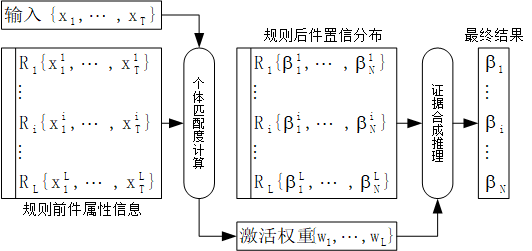
\includegraphics[width=\linewidth]{1brb.png}
    \caption{置信规则库证据合成推理流程}
\end{figure}

传统扩展置信规则库中每条规则激活权重的计算可看作两个置信分布之间相似度的计算,使用欧式距离对于第$i$个属性的个体匹配度度进行计算,将输入数据对应属性信息转换为置信分布形式后该属性个体匹配度为:
$$S_i^k=1-d_i^k=1-\sqrt{\sum_{j=1}^{J_i}(\alpha_{i,j}-\alpha_{i,j}^k)}$$
每个属性的个体匹配度度计算完成后,对所有属性进行聚合,合取规则形式下聚合函数为:
$$\alpha_k=\prod_{i=1}^{T_k}(S_i^k)^{\overline{\delta_i}},\overline{\delta_i}=\frac{\delta_i}{\max_{j=1,\cdots,T_k}\delta_j}$$
该条规则的激活权重由以下公式计算得到:
$$w_k=\frac{\theta_k\alpha_k}{\sum_{l=1}^L\theta_l\alpha_l}$$
规则权重归一化操作使得所有权重满足$0\leq w_k\leq 1,\sum w_k=1$。

使用置信分布相似度作为激活权重计算的方法已经不再适用于简化后的置信规则形式,为了进行有效的权重激活,本文使用高斯函数计算个体匹配度进行激活权重计算。
对于第$i$个属性信息,输入数据$X=(x_1,\cdots,x_{T_k})$与规则库中第$k$条规则$R_k:if(x_1^k , \cdots , x_{T_k}^k)then\{(D_1,\beta_1^k),\cdots,(D_N,\beta_N^k)\}$在该属性上个体匹配度度使用高斯函数计算为:
$$S_i^k=e^{-\frac{a(x_i-x_i^k)^2}{b}},a>0,b>0$$
其中正数参数$a$代表该属性对距离的敏感程度,距离不变时取值越大越敏感,属性匹配度越接近0。正数参数$b$代表该属性的权重,距离不变时取值越大属性重要度越低,属性匹配度越接近1。为了减少参数训练的数量,将参数$a$与$b$组合形成该属性对距离的敏感程度与属性权重相融合的属性辅助参数$\delta=\frac{a}{b}$,该属性个体匹配度可记为:
$$S_i^k=e^{-\delta(x_i-x_i^k)^2},\delta>0$$
对于合取规则置信规则库中单条规则激活权重由下式计算:
$$w_k=\frac{\theta_k\alpha_k}{\sum_{i=1}^L\theta_i\alpha_i},\alpha_k=\prod_{i=1}^{T_k}S_i^k=e^{-\sum_{i=1}^{T_k}\delta_i(x_i-x_i^k)^2},\delta_i>0$$

激活过程中参数$\delta$的取值可通过优化算法进行计算,也可以根据经验人为设定。对属性参数进行标准化去量纲处理后可直接设置参数$\delta=1$,即初始情况下属性不受距离敏感程度参数与属性权重参数影响。

传统置信规则库推理系统计算规则前件置信分布结构个体匹配度过程中,由于原始数据转换生成的规则在单个属性上至多仅有2个相邻的非零评价等级,导致不在这2个评价等级激活区域内的属性参数激活值为零。使用了改进的置信规则结构与基于高斯函数的激活权重计算方法后,任意规则的属性个体匹配度聚合后都是非零正值,避免了规则零激活问题影响推理系统性能。

规则权重计算完成后对所有规则进行合成并获得推理结果,首先将规则的置信分布转化为对应的可信度信息:
$$m_{j,k}=w_k\beta_j^k,j=1,\cdots,N$$
$$m_{D,k}=1-\sum_{j=1}^Nm_{j,k}=1-w_k\sum_{j=1}^{N}\beta_j^k$$
$$\overline{m}_{D,k}=1-w_k,\quad\widetilde{m}_{D,k}=w_k(1-\sum_{j=1}^N\beta_j^k)$$
其中$m_{j,k}$代表第$k$条规则在第$j$个结果属性上的可信度,$\overline{m}_{D,k}$代表第$k$条规则未分配给任何结果属性的可信度,
$\widetilde{m}_{D,k}$代表第$k$条规则结果参考属性不完备导致缺失的可信度,
不确定性可信度总和由$m_{D,k}=\overline{m}_{D,k}+\widetilde{m}_{D,k}$给出。
根据每条规则的可信度信息进行合成,得到第个$j$结果属性最终置信度结果:
$$m_j=k[\prod_{i=1}^L(m_{j,i}+m_{D,i})-\prod_{i=1}^Lm_{D,i}]$$
$$\overline{m}_D=n[\prod_{i=1}^L\overline{m}_{D,i}],\quad\widetilde{m}_D=k[\prod_{i=1}^Lm_{D,i}-\prod_{i=1}^L\overline{m}_{H,i}]$$
$$n=[\sum_{j=1}^N\prod_{i=1}^L(m_{j,i}+m_{D,i})-(N-1)\prod_{i=1}^Lm_{D,i}]^{-1}$$
$$\beta_j=\frac{m_j}{1-\overline{m}_D},\quad\beta_D=\frac{\widetilde{m}_D}{1-\overline{m}_D}$$
\subsection{改进的置信规则库推理系统复杂度分析}
本文提出的简化前件属性置信分布结构与使用高斯函数优化激活权重计算方法对置信规则库推理系统复杂度优化分为构建与推理两个部分。假设前件属性有$T$个,每个属性的候选数目$J$个,规则总数$L$条,一共$N$个结果评价等级。传统扩展置信规则库推理系统在构建过程中,生成每条规则的时间复杂度为$O(TJ)$,所有规则生成的时间复杂度为$O(LTJ)$。在推理过程中,对输入数据的转换与规则匹配度计算的时间复杂度为$O(LTJ)$,对规则进行证据合成推理的时间复杂度为$O(NL)$,推理过程的总复杂度为$O((N+TJ)\times L)$。

优化后的置信规则库推理系统由于简化了规则前件属性置信度分布结构,生成每条规则的时间复杂度降为$O(T)$,对输入数据的转换与规则匹配度计算的时间复杂度降为$O(LT)$,使得规则库构建与推理过程的总复杂度分别下降$O(LT)$和$O((N+T)\times L)$,同时避免了零激活问题。
\section{动量优化随机梯度下降法参数训练}
传统梯度法应用于置信规则库推理系统参数训练过程中受到规则属性偏导公式构造困难、训练步长受参数约束条件限制等问题。上文改进的置信规则库推理系统避免了传统置信规则系统求导困难的问题,同时通过引入指数归一化函数与线性整流函数避免参数训练过程中受到特定约束。最终采用动量优化随机梯度下降法进行参数训练,在降低计算资源消耗的同时提高了训练速度。
\subsection{改进的置信规则库推理系统梯度求解与可微分证明}
置信规则库推理的最终置信分布形式由公式给出,展开得到第$j$个结果属性数值:
$$\beta_j=\frac{m_j}{1-\overline{m}_D}$$
\begin{small}
    $$=\frac{\prod_{i=1}^L(m_{j,i}+m_{D,i})-\prod_{i=1}^Lm_{D,i}}{\sum_{t=1}^N\prod_{i=1}^L(m_{t,i}+m_{D,i})-(N-1)\prod_{i=1}^Lm_{D,i}-\prod_{i=1}^L\overline{m}_{D,i}}$$
\end{small}
本文推理系统的实现及相关实验均是在信息完整情况下进行,规则结果属性的置信分布中不包括不确定信息:
$$\sum_{i=1}^N\overline{\beta}_{ik}=1(k=1,\cdots,L),m_{D,i}=\overline{m}_{D,i},\widetilde{m}_{D,i}=0$$
完备情况下第$j$个结果属性表示为:
$$\beta_j=\frac{\prod_{i=1}^L(m_{j,i}+m_{D,i})-\prod_{i=1}^Lm_{D,i}}{\sum_{t=1}^N\prod_{i=1}^L(m_{t,i}+m_{D,i})-N\times\prod_{i=1}^Lm_{D,i}}$$
$$=\frac{\prod_{i=1}^L(\frac{m_{j,i}}{m_{D,i}}+1)-1}{\sum_{k=1}^N[\prod_{i=1}^L(\frac{m_{k,i}}{m_{D,i}}+1)-1]}$$
第$j$个结果属性未进行归一化的置信度表示为:
$$\overline{\beta}_j=\prod_{i=1}^L(\frac{m_{j,i}}{m_{D,i}}+1)-1,\beta_j=\frac{\overline{\beta}_j}{\sum_{k=1}^N\overline{\beta}_k}$$
将$m_{j,i}=w_i\beta_{j,i},m_{D,i}=1-w_i,w_i=\frac{\theta_i\alpha_i}{\sum_{k=1}^L\theta_k\alpha_k}$代入第$j$个未归一化置信度表达式中有:
$$\overline{\beta}_j=\prod_{i=1}^L(\frac{\theta_i\alpha_i\beta_{j,i}}{\sum_{k\neq i}^L{\theta_k\alpha_k}}+1)-1$$

根据高斯函数优化的规则权重激活过程,第$t$规则个体匹配度聚合值$\alpha_t$由该条规则前件属性信息与属性辅助参数的计算得到,设置最终置信度输出结果的损失函数表示为$loss=Loss(\beta_1,\cdots,\beta_N)$,根据多元复合函数求导链式法则,最终结果损失对第$t$条规则第$n$个前件属性求导为:
$$\frac{dloss}{dx_n^t}=\sum_{i=1}^N\sum_{j=1}^N \frac{loss}{d\beta_i}\frac{d\beta_i}{d\overline{\beta}_j}\frac{d\overline{\beta}_j}{d\alpha_t}\frac{d\alpha_t}{dx_n^t}$$
最终结果损失对第$n$个规则属性辅助参数求导为:
$$\frac{dloss}{d\delta_n}=\sum_{i=1}^N\sum_{j=1}^N\sum_{k=1}^L \frac{loss}{d\beta_i}\frac{d\beta_i}{d\overline{\beta}_j}\frac{d\overline{\beta}_j}{d\alpha_k}\frac{d\alpha_k}{d\delta_n}$$
最终结果损失对第$t$条规则的规则权重求导为:
$$\frac{dloss}{d\theta_t}=\sum_{i=1}^N\sum_{j=1}^N \frac{dloss}{d\beta_i}\frac{d\beta_i}{d\overline{\beta}_j}\frac{d\overline{\beta}_j}{d\theta_t}$$
注意到任意规则的第$j$个结束属性置信度仅与第$j$个未归一化的结果属性置信度相关,最终结果损失对第$t$条规则第$j$个结果置信分布求导为:
$$\frac{dloss}{d\beta_{j,t}}=\sum_{i=1}^N\sum_{j=1}^N\frac{dloss}{d\beta_i}\frac{d\beta_i}{d\overline{\beta}_j}\frac{d\overline{\beta}_j}{d\beta_{j,t}}$$

由于上述导数中除损失函数偏导外其他部分的偏导均存在$^{\ref{Appendix A}}$且连续$^{\ref{Appendix B}}$,当选定适当的损失函数后,最终结果损失对推理模型的所有参数都是可微分的,这为使用梯度法优化模型参数提供了条件。

根据上述导数与选定的损失函数,可以得到损失结果在模型各部分参数上的梯度。
损失函数在所有规则前件属性参数上的梯度是:
$$\nabla_{x}loss=\left[\begin{matrix}
            \frac{dloss}{dx_1^1} & \cdots & \frac{dloss}{dx_{T_k}^1} \\
            \vdots               & \ddots & \vdots                   \\
            \frac{dloss}{dx_1^L} & \cdots & \frac{dloss}{dx_{T_k}^L}
        \end{matrix}\right]$$
损失函数在所有规则属性辅助参数上的梯度是:
$$\nabla_{\delta}loss=\left[\begin{matrix}
            \frac{dloss}{d\delta_1} & \cdots & \frac{dloss}{d\delta_{T_k}}
        \end{matrix}\right]$$
损失函数在所有规则权重上的梯度是:
$$\nabla_{\theta}loss=\left[\begin{matrix}
            \frac{dloss}{d\theta_1} & \cdots & \frac{dloss}{d\theta_L}
        \end{matrix}\right]$$
损失函数在所有规则结果置信度分布上的梯度是:
$$\nabla_{\beta}loss=\left[\begin{matrix}
            \frac{dloss}{d\beta_{1,1}} & \cdots & \frac{dloss}{d\beta_{N,1}} \\
            \vdots                     & \ddots & \vdots                     \\
            \frac{dloss}{d\beta_{1,L}} & \cdots & \frac{dloss}{d\beta_{N,L}} \\
        \end{matrix}\right]$$

根据推理系统输出的置信分布与结果的损失函数对各部分参数的梯度,通过沿着负梯度方向更新参数进行模型优化。由于推理模型的参数有各自的约束条件,使用概率归一化函数和线性整流函数对受约束参数进行预处理避免训练过程中破坏特定的参数约束条件。
为了满足结果置信度和为1且各个置信度非负,使用指数归一化函数:
$$\beta_j^k=\frac{e^{\overline{\beta_j^k}}}{\sum_{i=1}^Ne^{\overline{\beta_i^k}}}(\sum_{i=1}^N\beta_j^k=1,\beta_j^k>0)$$
为了满足规则权重和属性辅助参数的非负约束,使用激活函数处理可能出现的负数情况,可使用线性整流函数SoftPlus:
$$\theta_n=f(\overline{\theta}_n),\delta_n=f(\overline{\delta}_n),f(x)=\ln(1+e^x)$$
\subsection{动量优化随机梯度下降法训练参数}
使用梯度下降法更新推理模型参数的优化过程由下面式子给出:
$$M_{new}(x,\beta,\theta,\delta)=M_{old}-\mu\nabla_{M_{old}}loss$$
其中梯度信息根据最终置信度分布的损失函数给出,学习率$\mu$即更新的步长信息需要设定。Chang\cite{a10}与Wu\cite{a12}给出的梯度训练过程中使用二分法在约束空间中迭代寻找最优步长,在梯度为0时还需添加摄动参数避免训练过程停滞。上文提到新的梯度参数模型使用了概率归一化函数和线性整流函数预处理受约束参数,在满足约束条件的同时对步长无限制要求。为了提高训练的速度,本文使用了动量优化随机梯度下降的方法。

随机梯度下降法\cite{a17}是一种在目标函数可微分条件下的迭代优化方法,使用数据的随机子集计算得到的梯度作为整个数据集梯度的估算值,在高维优化问题中降低了计算负担,更新步长由学习率与当前梯度大小综合决定,离最优解越远梯度越大,更新步长越大,离最优解越近则梯度越小,更新步长越小,使得更新步长能有效的适应不同的训练阶段并避免了传统梯度法中对步长参数的优化求解。

对于所有数据样本,其损失函数输出由所有样本的决定并根据其梯度更新模型参数
$$loss=\frac{1}{n}\sum_i^nLoss(\beta_i),M_{new}=M_{old}-\mu\nabla_{M_{old}}loss$$
随机梯度下降法随机选取了单个样本作为所有输出样本损失函数的预估值进行参数更新
$$M_{new}=M_{old}-\mu\nabla_{M_{old}}Loss(\beta_i)$$
避免训练过程中对每个样本的梯度进行计算,随机近似过程和凸优化理论\cite{a18}证明了选取适当学习率$\mu$时其收敛性,且在目标函数是凸函数或伪凸时随机梯度下降法几乎可以肯定的收敛到全局最小值。

随机梯度下降法的明显缺点是其更新方向完全依赖当前样本的梯度因而十分不稳定,本文采用了动量法\cite{a19}去优化随机梯度下降过程。动量法借用物理学中的动量概念,模拟运动时物体的惯性,即在更新过程中保留一定程度的历史梯度信息,与当前样本梯度结合,可以同时增加更新过程的稳定性与速度,并增强了摆脱局部最优解的能力。动量法使用加权融合历史更新参数与当前梯度信息作为本次更新参数:
$$v_t=\nu v_{t-1}+\mu\nabla_HM,M=M-v_t$$
将初始$v_0$设置为$0$,$\nu$一般设置为$0.9$。若当前梯度与之前更新方向相同,则动量法会使得模型在该梯度方向上加速参数更新过程,提高训练的速度。若当前梯度方向与之前更新方向相反,则动量法可以抑制本次梯度信息造成的模型参数震荡。
\section{实验与结果}
本文引入非线性多极值函数及多个公共数据分类集,研究验证梯度训练下改进的置信规则库推理模型的训练效率与精确度。实验中模型使用TensorFlow 2搭建,运行于Intel$^{\copyright}$ Core$^{\texttrademark}$ i5 8500@3GHz,16GB内存,Nvidia 1060 6GB显卡,Ubuntu 20.04操作系统。
\subsection{非线性函数拟合}
Liu\cite{a15}证明了置信规则库可以逼近任意函数,本节通过引入一个非线性多极值函数进行训练验证模型的推理性能。
非线性多极值函数如下所示:
$$f(x)=e^{-(x-2)^2}+0.5e^{-(x+2)^2},-5\leq x\leq 5$$
在其定义域上均匀的选取$1000$组数据作为训练数据,使用均方误差作为损失函数,由函数曲线图所显示的各个极值点可设置规则库结果属性评价等级与相应的效用值:
$$\{D_1,D_2,D_3,D_4,D_5\}=\{-0.5,0,0.5,1,1.5\}$$
在规则构建过程中,通过随机生成定义域范围内的点作为规则前件属性信息,同时使用随机正态分布生成规则的置信分布并使用指数归一化函数进行预处理,设定规则数目为$16$,初始属性辅助参数与初始规则权重均设置为$1$。进行梯度训练时学习率$\mu=0.01$,动量优化参数$\nu=0.9$,随机梯度下降训练过程中每批次样本数量为$64$,对数据集训练$1000$批次后终止。与之对比的拓展置信规则库使用相同的参数并从函数曲线上随机抽取数据点作为规则库规则信息,同时为了比对更大批次下普通随机梯度法的效果,增加了$2000$批次训练的随机梯度法模型。

对比图2拓展置信规则库、图3使用随机梯度下降法训练的置信规则库与图4动量优化梯度法训练的置信规则库上不同用的推理效果,证明了梯度下降法能有效的提高推理系统的精确度。
\begin{figure}
    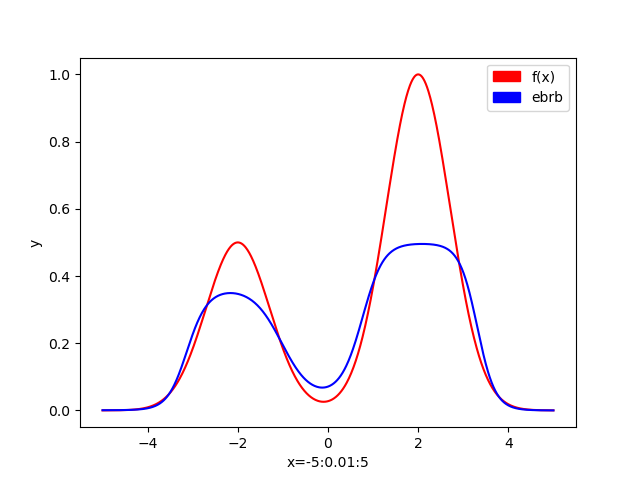
\includegraphics[width=\linewidth]{ebrb_fit.png}
    \caption{拓展置信规则库拟合图像}
\end{figure}

\begin{figure}
    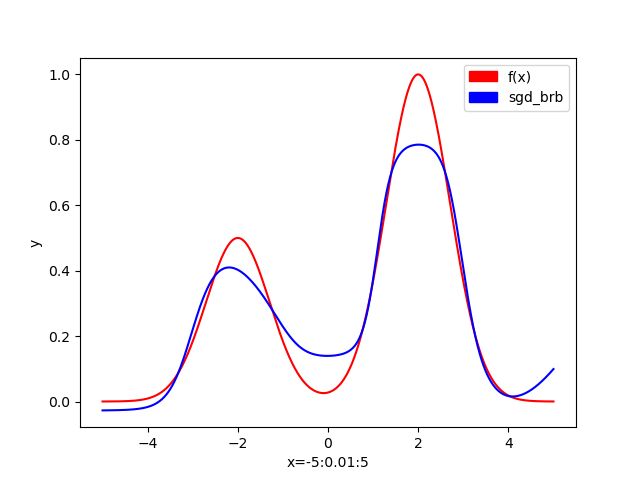
\includegraphics[width=\linewidth]{sgd_brb_fit.png}
    \caption{随机梯度法训练的拓展置信规则库拟合图像}
\end{figure}

\begin{figure}
    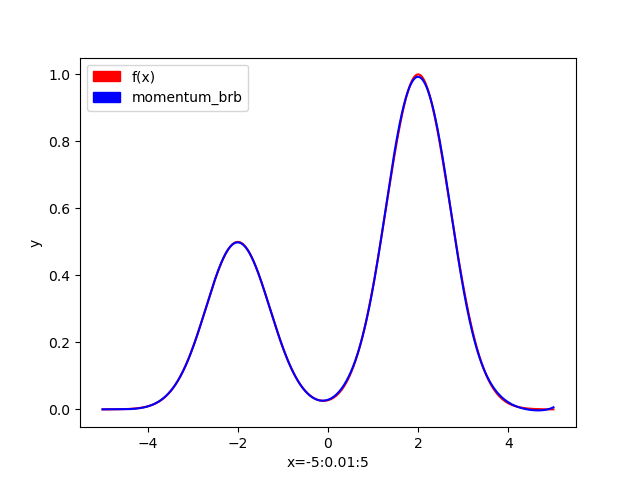
\includegraphics[width=\linewidth]{momentum_brb_fit.png}
    \caption{动量优化随机梯度法训练的拓展置信规则库拟合图像}
\end{figure}

图5与图6分别为随机梯度法和动量优化随机梯度法在每批次训练样本上的损失函数值,可以发现动量优化的随机梯度下降法训练速度极快,在第10秒均方差损失就下降到$2\times10^{-5}$水平。
\begin{figure}
    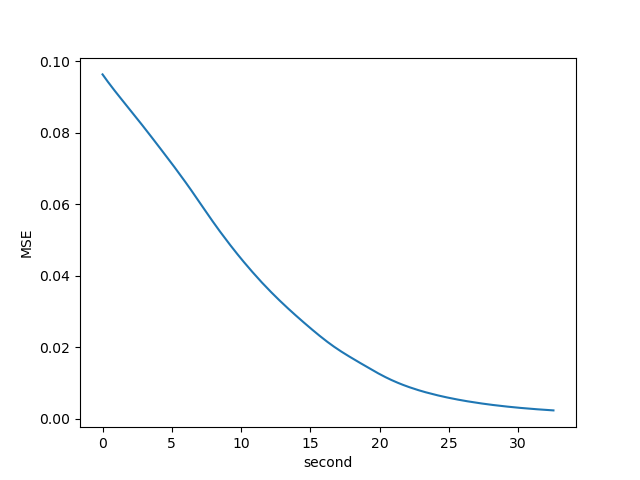
\includegraphics[width=\linewidth]{sgd_loss.png}
    \caption{随机梯度法训练过程中每批次样本上的损失函数值}
\end{figure}

\begin{figure}
    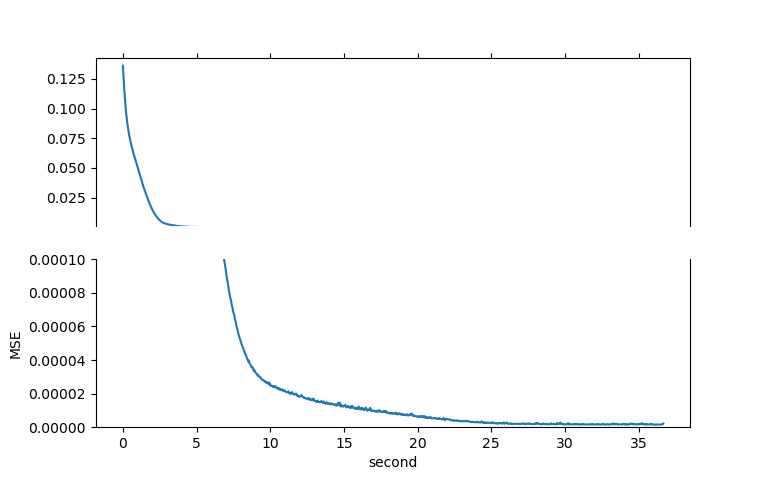
\includegraphics[width=\linewidth]{momentum_loss.png}
    \caption{动量优化的随机梯度法训练过程中每批次样本上的损失函数值}
\end{figure}

表1中对比了本文方法与Fmincon方法、Chen的局部优化参数训练方法、Wang的专家干预差分进化法及Li的布谷鸟搜索法,可以发现新方法无论在精度还是速度上都较以往方法有极大提升。在相同训练参数设置的前提下,随机梯度下降法损失函数下降较为平滑,最终的均方误差较大,当提升了训练批次后均方误差结果可以达到动量优化后的梯度法的水平。
\begin{table}
    \centering
    \caption{不同参数训练方法训练结果}
    \small
    \begin{tabular}{ccc}
        \toprule
                      & MSE均方误差            & 运行时间 \\
        \midrule
        Fmincon       & 5.16$\times 10^{-5}$   & 496.71   \\
        Chen-BRB      & 6.3228$\times 10^{-5}$ & -        \\
        Wang-BRB      & 3.9284$\times 10^{-5}$ & 386.63   \\
        Li-BRB        & 3.3322$\times 10^{-5}$ & 357      \\
        SGD-BRB(1000) & 5.410$\times 10^{-3}$  & 35.38    \\
        SGD-BRB(2000) & 1.2024$\times 10^{-5}$ & 66.06    \\
        momentum-BRB  & 1.3691$\times 10^{-6}$ & 37.72    \\
        \bottomrule
    \end{tabular}
\end{table}

\subsection{公共分类数据集测试}
本文从UCI上选择了9种较为常见的公共分类数据集进行测试,数据集详细信息见表2。使用10折交叉验证实验方法生成训练数据与测试数据,并重复实验10次求平均实验结果减少误差波动。模型使$32$条规则,为了简化前件属性参数生成过程,对训练数据所有属性信息进行标准化去量纲预处理,并使用标准正态分布随机生成所有前件属性参数值,同时使用标准正态分布随机生成结果置信分布并进行指数归一化预处理,初始化所有属性辅助参数与规则权重为$1$。梯度训练过程中批次大小设置为$128$,训练$1000$批次后终止,学习率与动量优化参数分别设置为$0.01$与$0.9$,使用交叉熵作为分类结果的损失函数。表3中使用准确率作为衡量分类结果评价指标,统计对比本文方法与SRA-BRB\cite{a21}、MVP-BRB\cite{a22}与BA-BRB\cite{a23}这几种置信规则库系统的分类效果。
\begin{table}
    \centering
    \caption{分类数据集信息}
    \begin{tabular}{cccc}
        \toprule
        数据集      & 类别数目 & 属性数目 & 样本数目 \\
        \midrule
        iris        & 3        & 4        & 150      \\
        wine        & 3        & 13       & 178      \\
        diabetes    & 2        & 8        & 768      \\
        ecoli       & 8        & 7        & 336      \\
        seeds       & 3        & 7        & 210      \\
        yeast       & 10       & 8        & 1484     \\
        transfusion & 2        & 4        & 748      \\
        \bottomrule
    \end{tabular}
\end{table}

从表3中可以发现本文方法在超过一半的数据集上超越了其他置信规则库推理方法,仅在ecoli与transfusion两个数据集上未能超越现有方法,其余数据集上均超过或达到其他推理方法的水平且平均排名结果最高。验证了本文方法在推理精度与效率上均超越了以往方法。
\begin{table}
    \centering
    \caption{分类数据集实验结果}
    \small{
        \begin{tabular}{ccccc}
            \toprule
            数据集       & SRA-BRB  & MVP-BRB  & BA-BRB   & 本文方法 \\
            \midrule
            iris         & 95.10(4) & 95.87(2) & 95.26(3) & 96.50(1) \\
            wine         & 96.85(3) &          & 97.02(2) & 97.44(1) \\
            diabetes     & 71.71(4) & 72.59(3) & 72.80(2) & 73.64(1) \\
            ecoli        & 84.85(3) & 85.61(1) &          & 85.43(2) \\
            seeds        & 91.24(4) & 92.38(3) & 93.95(2) & 94.02(1) \\
            yeast        & 56.85(4) & 57.49(3) & 58.63(2) & 59.49(1) \\
            transfusion  &          & 80.36(1) &          & 79.45(2) \\
            \midrule
            average rank & 3.66     & 2.166    & 2.2      & 1.28     \\
            \bottomrule
        \end{tabular}}
\end{table}

\section{结束语}
针对以往扩展置信库推理系统中构建规则消耗计算资源,规则权重零激活问题,本文提出通过简化前件属性置信分布结构,使用高斯函数优化激活权重计算过程,同时使用动量优化的随机梯度下降方法训练模型参数解决对应问题并提高推理性能。该方法结合结构优化与参数训练两个方面,通过优化结构使快速的梯度训练方法能够应用,最终提升了整个系统的推理效率。该方法具有良好的扩展性能,在实验分析中,本文方法在多个数据集上都较以往方法具有更高的推理性能。在接下来的工作中,以这种简化模型与快速参数训练的方法将使得多个推理模型进行集成学习成为可能的研究方向。


\nocite{*}

\bibliographystyle{cjc}
\bibliography{example}

\newpage



\appendix

\section{置信规则库推理模型偏导求解}
\label{Appendix A}
第$i$个结果属性置信度$\beta_i$对第$j$个未归一化结果属性置信度$\overline{\beta}_j$求导为:
$$\frac{d\beta_i}{d\overline{\beta}_j}=
    \left\{
    \begin{aligned}
        \frac{\sum_{k\neq j}^N\overline{\beta}_k}{(\sum_{k=1}^N\overline{\beta}_k)^2},j=i \\
        -\frac{\beta_i}{(\sum_{k=1}^N\overline{\beta}_k)^2},j\neq i
    \end{aligned}
    \right.$$
第$j$个未归一化结果属性置信度对第$t$条规则的个体匹配度聚合值求导为:
$$\frac{d\overline{\beta}_j}{d\alpha_t}=\frac{\theta_t\beta_{j,t}}{\sum_{k\neq t}^L\theta_k\alpha_k}\prod_{i=1,i\neq t}^L(\frac{\theta_i\alpha_i\beta_{j,i}}{\sum_{k\neq i}^L{\theta_k\alpha_k}}+1)$$
$$+\sum_{l=1,l\neq t}^L(-\frac{\theta_l\alpha_l\beta_{j,l}\theta_t}{(\sum_{k\neq l}^L\theta_k\alpha_k)^2}\prod_{i=1.i\neq l}^L(\frac{\theta_i\alpha_i\beta_{j,i}}{\sum_{k\neq i}^L{\theta_k\alpha_k}}+1))$$
第$t$条规则个体匹配度聚合值对相应规则的第$n$个前件属性参数求导为:
$$\frac{d\alpha_t}{dx_n^t}=-2\delta_n(x_n-x_n^t)e^{-\sum_{i=1}^{T_k}\delta_i(x_i-x_i^t)^2}$$
第$t$条规则个体匹配度聚合值对第$n$个规则属性辅助参数求导为:
$$\frac{d\alpha_t}{d\delta_n}=-(x_n-x_n^t)^{2}e^{-\sum_{i=1}^{T_k}\delta_i(x_i-x_i^t)^2}$$
第$j$个未归一化结果属性置信度对第$t$条规则的规则权重求导为:
$$\frac{d\overline{\beta}_j}{d\theta_t}=\frac{\alpha_t\beta_{j,t}}{\sum_{k\neq t}\theta_k\alpha_k}\prod_{i=1,i\neq t}^L(\frac{\theta_i\alpha_i\beta_{j,i}}{\sum_{k\neq i}{\theta_k\alpha_k}}+1)$$
$$+\sum_{l=1,l\neq t}^L(-\frac{\theta_l\alpha_l\beta_{j,l}\alpha_t}{(\sum_{k\neq l}\theta_k\alpha_k)^2}\prod_{i=1.i\neq l}^L(\frac{\theta_i\alpha_i\beta_{j,i}}{\sum_{k\neq i}{\theta_k\alpha_k}}+1))$$
第$j$个未归一化结果属性置信度对第$t$条规则对应第$j$个结果属性置信度求导为:
$$\frac{d\overline{\beta}_j}{d\beta_{j,t}}=\frac{\theta_t\alpha_t}{\sum_{k\neq j}\theta_k\alpha_k}\prod_{i=1,i\neq t}^L(\frac{\theta_i\alpha_i\beta_{j,i}}{\sum_{k\neq j}\theta_k\alpha_k}+1)$$

\section{置信规则库推理模型可微分证明}
\label{Appendix B}
置信规则库推理过程是一个多元复合函数过程,根据多元复合函数可微分条件,各中间函数皆需满足微分条件,同时对各个变量的偏导要求存在且连续。根据损失结果对第$t$条规则第$n$个前件属性的导数表达式:
$$\frac{dloss}{dx_n^t}=\sum_{i=1}^N\sum_{j=1}^N \frac{loss}{d\beta_i}\frac{d\beta_i}{d\overline{\beta}_j}\frac{d\overline{\beta}_j}{d\alpha_t}\frac{d\alpha_t}{dx_n^t}$$
当选择损失函数的导数存在并连续时,任选一条求导路径$\frac{dloss}{d\beta_i}\frac{d\beta_i}{d\overline{\beta}_j}\frac{d\overline{\beta}_j}{d\alpha_t}\frac{d\alpha_t}{dx_n^t}$进行连续证明。


对过程$\beta_i(\overline{\beta}_1,\cdots,\overline{\beta}_N)$中对$\overline{\beta}_j$的偏导$\frac{d\beta_i}{d\overline{\beta}_j}$进行连续性证明:
$$\frac{d\beta_i}{d\overline{\beta}_j}(\overline{\beta}_j)=
    \left\{
    \begin{aligned}
        \frac{\sum_{k\neq j}^N\overline{\beta}_k}{(\sum_{k=1}^N\overline{\beta}_k)^2},j=i \\
        -\frac{\beta_i}{(\sum_{k=1}^N\overline{\beta}_k)^2},j\neq i
    \end{aligned}
    \right.$$
由于上述偏导具有初等函数形式,且$\overline{\beta}_j\in(0,+\inf)$,该偏导在其定义域上是连续的。

对过程$\overline{\beta}_j(\alpha_1,\cdots,\alpha_L,\theta_1,\cdots,\theta_L,\beta_{j,1},\cdots,)$中对$\alpha_t$的偏导为$\frac{d\overline{\beta}_j}{d\alpha_t}$进行连续性证明:
$$\frac{d\overline{\beta}_j}{d\alpha_t}(\alpha_t)=\frac{\theta_t\beta_{j,t}}{\sum_{k\neq t}^L\theta_k\alpha_k}\prod_{i=1,i\neq t}^L(\frac{\theta_i\alpha_i\beta_{j,i}}{\sum_{k\neq i}^L{\theta_k\alpha_k}}+1)$$
$$+\sum_{l=1,l\neq t}^L(-\frac{\theta_l\alpha_l\beta_{j,l}\theta_t}{(\sum_{k\neq l}^L\theta_k\alpha_k)^2}\prod_{i=1.i\neq l}^L(\frac{\theta_i\alpha_i\beta_{j,i}}{\sum_{k\neq i}^L{\theta_k\alpha_k}}+1))$$
同样由于上述偏导具有初等函数形式,且$\alpha_t\in(0,1]$,该偏导在其定义域上是连续的。

对过程$\alpha_t(x_1^t,\cdots,x_{T_k}^t,\delta_1,\cdots,\delta_{T_k})$中对$x_n^t$的偏导为$$\frac{d\alpha_t}{d\delta_n}=-(x_n-x_n^t)^{2}e^{-\sum_{i=1}^{T_k}\delta_i(x_i-x_i^t)^2}$$
同样具有初等函数形式且$x_n^t\in(-\inf,+\inf)$,该偏导在其定义域上是连续的。

由于路径$\frac{dloss}{d\beta_i}\frac{d\beta_i}{d\overline{\beta}_j}\frac{d\overline{\beta}_j}{d\alpha_t}\frac{d\alpha_t}{dx_n^t}$上各部分中间偏导均存在且在各自定义域上连续,根据连续函数四则运算法则,其连乘得到路径偏导同样连续。由于任意路径偏导连续,最终求和得到偏导表达式仍具有连续性质。由于置信规则库推理系统中激活与推理部分均由初等函数构成,各参数不同路径的偏导都具有相似的连续性质,可证明当选取合适损失函数时损失结果对推理系统各个参数是可微分的。


\makebiographies


\end{document}
